% Introduction
This chapter discusses the security design solution based on the security requirements described in section \ref{subsec:sec-req}. The chapter will start with the system architecture design, followed by security designs for each security requirement discussed per category. The design will be illustrated using figures and code implementations in Python and TypeScript for the back-end and front-end respectively.

\section{Software Architecture Design}
\begin{figure}
    \centering
    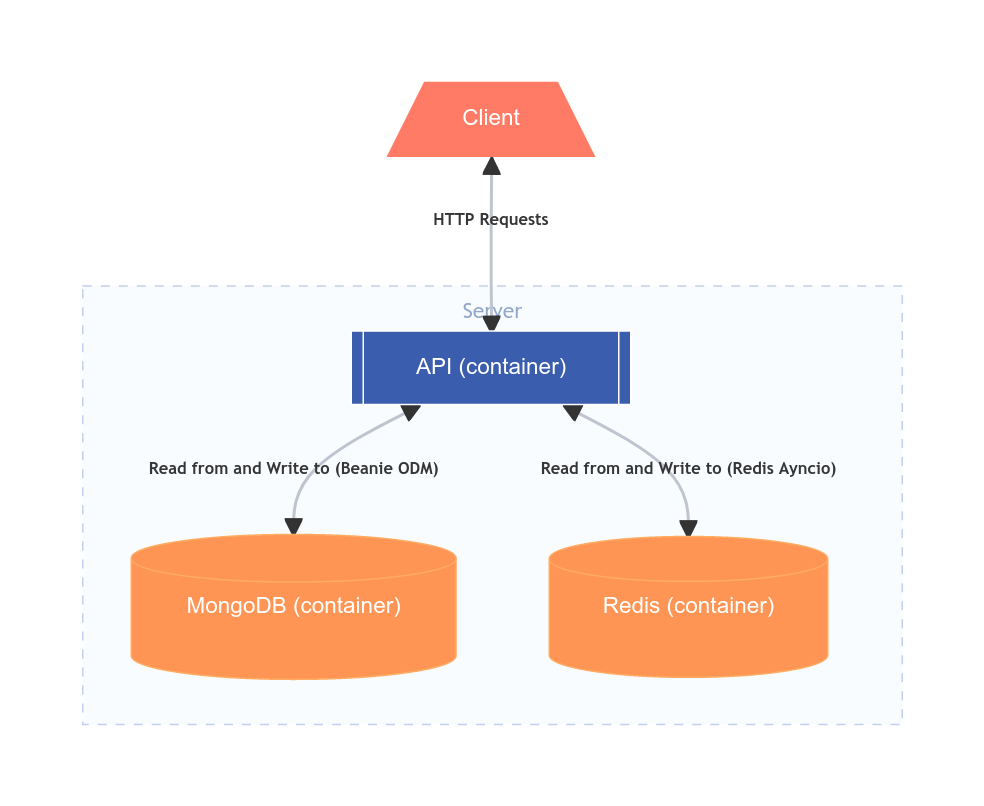
\includegraphics[width=\textwidth]{../../img/chapter-4/system-arch.png}
    \caption{System-Architecture Overview}
    \label{fig:sys-arch}
\end{figure}

\section{Users, Authentication and Authorization}
CheFeed requires users to be authenticated and authorized to perform certain actions such as posting recipes or posting reviews as described in the users stories. Users are stored ina MongoDB database whilst their tokens are stored in a Redis database. Each time a user starts a new session, a random bearer token is generated on the server-side and stored in Redis. The token is sent in the response body when a user starts the session for the first time to give the user authorization for protected resources, therefore the client must store that token securely for future reference. Figure \ref{fig:auth-flow} illustrates the design of the authentication flow.

\begin{figure}
    \centering
    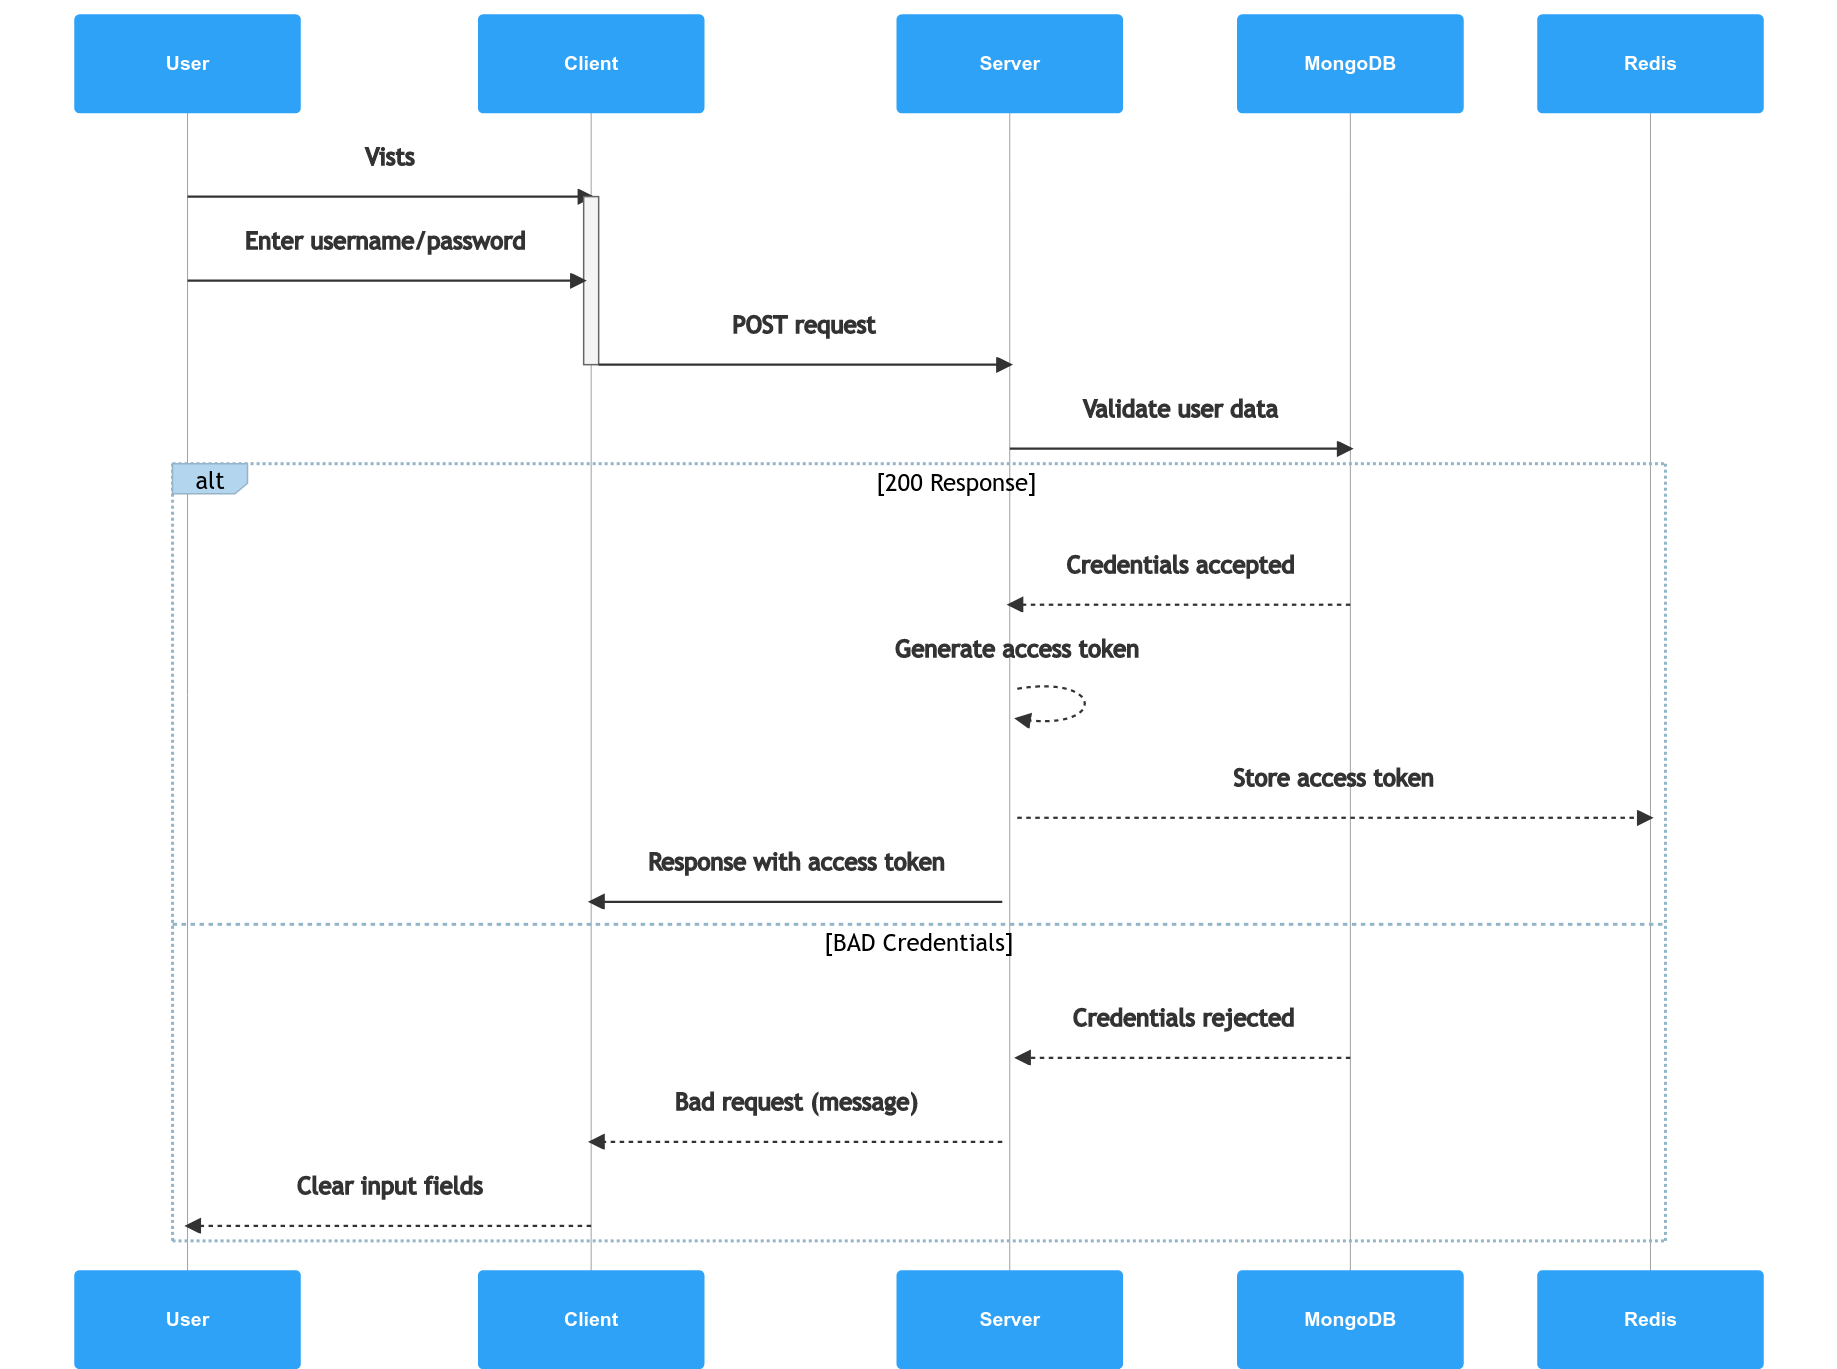
\includegraphics[width=\textwidth]{../../img/chapter-4/auth-flow.png}
    \caption{Authentication flow}
    \label{fig:auth-flow}
\end{figure}

\subsection{Data Storage and Privacy}
The verifications 2.1, 2.2, 2.3, 2.5, 2.6, 2.7 in Table \ref{tab:sec-req} describes the requirements for \say{Data Storage and Privacy}.

\subsubsection{Local Storage for Sensitive Data}
As illustrated in Figure \ref{fig:auth-flow}, random authorization tokens are generated for each user session. These tokens need be stored securely on the client side. Ideally, sensitive data such as a user token, should be stored off device, or not stored at all. However,  asking the user to input complex passwords each time the app starts is not a great usability feature. To avoid this, CheFeed ensures the token is stored securely on the local device. With React Native, expo provides the \textit{SecureStore} API to encrypt and securely store key-value pairs locally on the device. Its implementation can be seen in Listing \ref{lst:secure-store}

\subsection{Authentication and Session Management}
SKF generated seven security requirements for the category \say{Authentication and Session Management Requirements}. For the development of the users and authentication feature, we relied on the third party library \textit{fastapi-users} for FastAPI. The library describes itself as a \say{ready-to-use and customizable users management for FastAPI}. It includes features such as an extensible base user model, ready-to-use users and authentication routes, pluggable password validation, a customizable database backend and more. This speeds up development time and prevents developers the need to reinvent mechanisms that are common in modern software development. 

\subsubsection{Authentication Design}
CheFeeds provides a resource to allow users to authenticate using an email and password combination. In this case, the mobile client needs to send the correct email and password in proper format to the resource where the request is validated. An overview of all the implemented authentication resources are described in Table \ref{tab:auth-resources}

\begin{table}
    \centering
    \caption{Authenication Resources}
    \label{tab:auth-resources}
    \begin{tabulary}{1.0\textwidth}{|L|L|L|}
        \hline
        \textbf{Method} & \textbf{Resource} & \textbf{Protected} \\ 
        \hline
        POST & /auth/login & \textit{No} \\
        \hline
        POST & /auth/logout & \textit{Yes} \\
        \hline
        POST & /auth/register & \textit{Yes} \\
        \hline
    \end{tabulary} 
\end{table}

\paragraph{Fastapi-Users Authentication Implementation} Implementing the authentication resources in fastapi-users is fairly straight forward. It includes the implementation of the user model, database, transport (how the token will be carried over the request), strategy (how the token is generated and secured), and including the routes. Listing \ref{lst:auth} shows a critical part of the authentication mechanism. It shows the implementation of the authentication transport and strategy implemented in the \textit{auth\_backend.py} module. 

\subparagraph{Bearer Transport} CheFeed implements the bearer transport method as it is easy to read and set in every request. However, the token needs to be stored manually in the client side. Nevertheless, the fastapi-users documentation suggest the bearer method when implementing a mobile application or a pure REST API as is the case for CheFeed. Therefore, it is an appropriate choice.

\subparagrah{Redis Strategy} There are several ways to generate and secure tokens with fastapi-users. CheFeeds implemented a redis strategy as is illustrated in Figure \ref{fig:sys-arch} and shown in Listing \ref{lst:auth}. Redis has the benefit of being secure, performant, and the functionality of invalidating the token on the server-side.


\begin{lstlisting}[language=Python, caption={auth\_backend.py}, label={lst:auth}, float]
import redis.asyncio
from fastapi_users.authentication import (
    AuthenticationBackend,
    BearerTransport,
    RedisStrategy)

redis = redis.asyncio.from_url(
    settings.REDIS_URL, 
    decode_responses=True)

bearer_transport = BearerTransport(
    tokenUrl='auth/login')

def get_redis_strategy() -> RedisStrategy:
    return RedisStrategy(
        redis, 
        lifetime_seconds=31557600)

auth_backend = AuthenticationBackend(
    name='Redis',
    transport=bearer_transport,
    get_strategy=get_redis_strategy
)
\end{lstlisting}

\subsection{Cryptography Design}


